\documentclass{article}
\usepackage{amsmath}
\usepackage{amssymb}
\usepackage{graphicx}
\usepackage{tikz,pgfplots}
\usepackage[utf8]{inputenc}
\usepackage{changepage}
\pgfplotsset{compat=1.11}


%Primero será necesario inicializar el documento%
%Inicio documento%
\begin{document}
%Ahora se comenzará a hacer la portada para comenzar con el trabajo%
%Inicio Portada%
   \begin{titlepage}
       %Centraremos el texto para comenzar%
       \centering
       %Fotografía del escudo de la escuela%
       {
\includegraphics[width=0.2\textwidth]{logo.png} \par}
       %Texto de la portada%
       {\bfseries\LARGE\textit{Universidad Nacional Autónoma de México}\par}
       %Vspace será el espacio que existe entre un párrafo y el siguiente%
       \vspace{1cm}


       {\scshape\Large Facultad de Estudios Superiores Acatlán \par}
       \vspace{3cm}


       {\scshape\Huge Ejercicio 3: Métodos Abiertos}
       \vspace{3cm}


       {\slshape\Large Materia: Métodos Numéricos 1 \par}
       \vfill


       {\Large Autor: Díaz Valdez Fidel Gilberto \par}
       {\Large Número de cuenta: 320324280 \par}


       \vfill
       {\Large Septiembre 2023 \par}


   \end{titlepage}


\section{Propósito}
Hacer uso del método numérico de Newton-Raphson para aplicarlo en la problemática a resolver para así encontrar una solución satisfactoria al problema además de ganar soltura y experiencia tanto en la utilización de este método, como en la aplicación de otras dependiendo de lo que se requiera y las herramientas que se dispongan.


\section{Instrucciones}
Según la ecuación de Van der Waals para algún gas real encontrar el valor de $V$.


El gas en cuestión es cloruro de estaño y la ecuación la siguiente:
$$ (P+\frac{a}{V^2})(V-b)=RT $$


Los datos proporcionados:
\begin{itemize}
   \item $P$ = Presión en $atm$ (atmosférica) = $50 atm$
   \item $T$ = Temperatura en $K$ (Kelvin) = $68$ $C$º
   \item $R$ = $0.08205 atm-L/(gmolK)$
   \item $V$ = Volumen molar del gas en $L/mol$
   \item $a$ = Constante del cloruro de estaño = $27.27$
   \item $b$ = Constante del cloruro de estaño = $0.1642$
\end{itemize}


\section{Fórmula}
El siguiente paso es sustituir los valores que nos proporcionan en la misma ecuación.


Pero antes de hacer esto es necesario pasar la temperatura a Kelvin ya que se nos fue proporcionada en Celsius.


La fórmula es esta: $68$Cº$+273.15K= 341.15K$




El resultado de sustituir los datos es:
$$ (50+\frac{27.27}{V^2})(V-0.1642)=(0.08205)(341.15) $$
Lo que nosotros realmente necesitamos es el valor de $V$ que satisfaga la ecuación y esto se podría hacer al resolver la ecuación pero si suponemos el caso en donde es muy complicado resolverla como normalmente lo hacemos por medio de algebra, aquí es donde entra el método de Newton-Raphson o secante.


Lo que realmente necesitamos es que se satisfaga la ecuación por lo que primero la igualamos a cero teniendo como resultado lo siguiente:
$$ (50+\frac{27.27}{V^2})(V-0.1642)-27.9913575=0$$
Como mencione anteriormente, sería necesario encontrar el valor de $V$ y esto se podría realizar al solo despejar, es decir, encontrar el valor de $V$ que cumple que realizando las operaciones correspondientes con los datos proporcionados se cumpla que el resultado final de las operaciones es 0.


Es decir buscar la $V$ que haga que el resultado sea cero, casi como si se tratará de una función, pero como ya mencionamos buscamos hacer uso del método de Newton-Raphson por lo que necesitamos una función que evaluar en diferentes puntos hasta encontrar la $V$ que nos arroje una raíz, es decir, que haga que el resultado de la ecuación sea 0.


Haciendo este análisis y teniendo la ecuación igualada a cero podemos afirmar que la función que utilizaremos para encontrar el valor de $V$ que nos devuelve una raíz es:
$$f(x) = (50+\frac{27.27}{x^2})(x-0.1642)-27.9913575$$




Teniendo la función a utilizar para el método ya estamos en condiciones de graficar.


\section{Gráfica}


\begin{figure}[h]
   \centering
   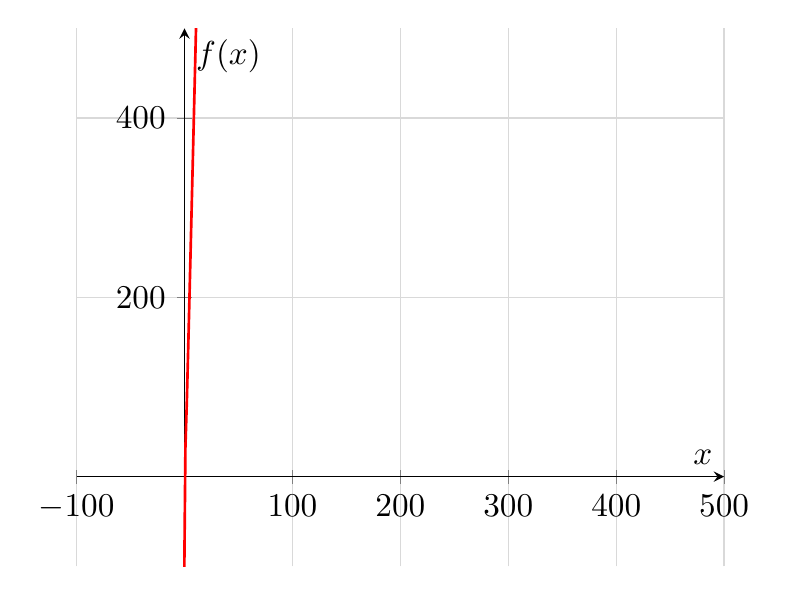
\begin{tikzpicture}[scale=1.2]
       \begin{axis}[
         axis lines= middle,
           xlabel=$x$,
           ylabel=$f(x)$,
           xmin=-100, xmax=500,   % Amplía los límites del eje x
           ymin=-100, ymax=500,     % Ajusta los límites del eje y según tus datos
           grid=major,  % Activa la cuadrícula
           grid style={gray!30},  % Estilo de la cuadrícula
           ]
           \addplot[domain=-20:500, samples=400, color=red, thick]{(50+(27.27/x^2))*(x-0.1642)-27.9913575};
       \end{axis}
   \end{tikzpicture}
  
\end{figure}


Así es como se comporta la función de manera general, agrande la escala para poder ser capaces de apreciar cómo se comporta ya que muy de cerca tiene parecido a una simple recta.
La función más de cerca para apreciar su raíz es la siguiente:
      
\begin{figure}[h]
   \centering
   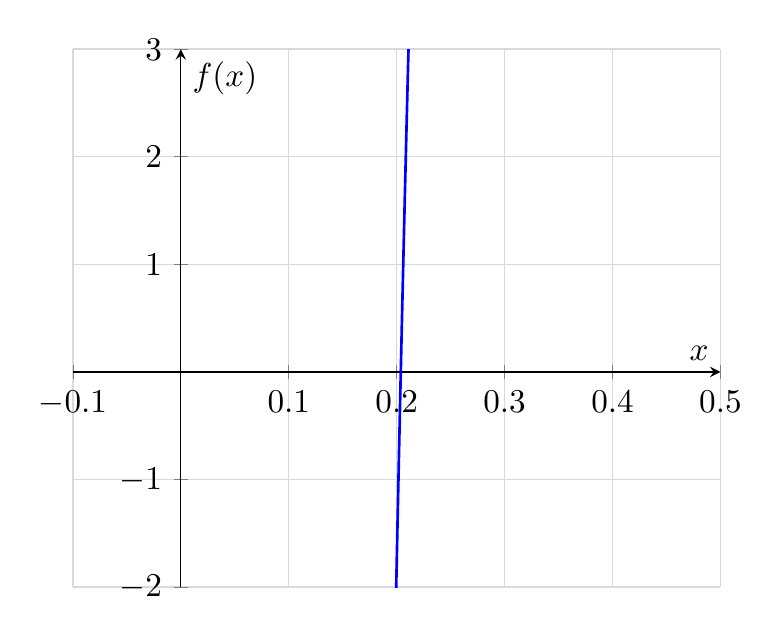
\begin{tikzpicture}[scale=1.2]
       \begin{axis}[
           axis lines=middle,
           xlabel=$x$,
           ylabel=$f(x)$,
           xmin=-0.1, xmax=0.5,   % Límites del eje x
           ymin=-2, ymax=3,   % Límites del eje y
           xtick={-0.1,0, 0.1, 0.2, 0.3, 0.4, 0.5}, % Marcas en el eje x
           ytick={-2, -1, 0, 1, 2,3}, % Marcas en el eje y
           grid=major,  % Activa la cuadrícula
           grid style={gray!30},  % Estilo de la cuadrícula
       ]
       % Función a graficar
       \addplot[domain=0.1:0.3, samples=1000, color=blue, thick]{(50+(27.27/x^2))*(x-0.1642)-27.9913575};
       \end{axis}
   \end{tikzpicture}
\end{figure}


\section{Intervalo de solución}
Como se puede ver en la segunda gráfica la raíz se encuentra entre $0.2$ y $0.3$ por lo que ese será el intervalo que escogeremos para encontrar la raíz: $[0.2, 0.3]$.
También debemos elegir la tolerancia al error relativo porcentual además del intervalo inicial ya elegido, en este caso la tolerancia será $0.0001$%


\section{Implementación del método de Newton-Raphson y de la Secante}
\subsection{Newton-Raphson}
Sabemos de igual manera que el método de Newton solo necesita de un solo valor para comenzar, en este caso utilizaremos el $0.2$ del intervalo elegido para evaluar, ya que como se ve en la gráfica, podría parecer que si se evalúa la función en un valor más pequeño este vaya hasta el infinito positivo y si no es el caso
podría llegar muy lejos a un valor difícil tanto de entender como de implementar en el método, pero en el caso del $0.2$ se puede observar una cercanía muy evidente con la raíz.


El paso siguiente será calcular su derivada para poder hacer uso del método, para calcularla solo utilizaremos
a GeoGebra que nos brinda facilidades para calcular derivadas según una función ingresada, una vez terminado este
paso la derivada es: $$f`(x)= \frac{12500000x^3-6817500x+2238867}{250000x^3}$$


Una vez que se tiene la derivada solo será necesario comenzar a evaluar la $f(x)$ y la $f`(x)$ para después con
estos datos calcular la nueva $x$ a evaluar, se calcula con la siguiente fórmula: $$x_{k+1}=x_k-\frac{f(x_k)}{f`(x_k)}$$


Por lo tanto el cálculo para el nuevo elemento es: $$x_{k+1}=0.2-\frac{0.66679245}{487.6835}= 0.01522110658$$


Con este nuevo dato se continuará a calcular la función y la derivada con este valor así se seguirá hasta llegar a
la raíz aproximada, esto si es que no tuvimos la mala suerte de encontrarnos en un caso patológico, si llegase a ser
En el caso solo necesitaremos elegir otro dato inicial y comenzar desde cero el proceso.


Esto se puede realizar desde una hoja de cálculo, solo necesitamos configurarla con la fórmula para calcular la imagen
de la función y de la derivada según un dato dado y el resultado será una tabla de iteraciones que se ve de la siguiente
manera:


\begin{table*}[h] 
   \begin{adjustwidth}{-1.5cm}{0cm}
       \resizebox{16cm}{!}{
           \begin{tabular}{| c | c | c | c | c | c |}
               \hline
               $k$ & $x_k$ & $f(x)$ & $f'(x)$ & $E_{r\%}$ & Tolerancia \\ \hline
                 0 &0.2 & -1.79470755& 487.6835 & & \\ \hline
                 1 &0.2036800661 &-0.06564569939 &452.5088452 &1.8067\% & Continuar\\ \hline
                 2 & 0.2038251366& -0.00009623698927&451.1828243 &0.0711\% &Continuar \\ \hline
                 3 & 0.2038253499&-0.0000000002075850603 &451.1808779 & 0.0001\%& Parar \\ \hline
           \end{tabular}
       }
   \end{adjustwidth}
\end{table*}


\subsection*{Conclusión}
Como se puede observar la raíz a la que se aproximo es: $0.2038253499$.


El punto de paro se dio gracias a la incumplición de la tolerancia, pero observando el comportamiento de la tabla y la
diferencia cada vez menor con la iteración anterior, es muy probable y seguro que en la siguiente se llegaría a la raíz
exacta sino nos hubiéramos detenido por la tolerancia al error.


\subsection{Secante}
Para este método si es necesario partir de dos datos iniciales para calcular el nuevo dato a utilizar, pero de igual manera
es importante mencionar que no será necesario en este método que los datos encierren a la raíz, por lo que la manera de
elegir el próximo $x$ no tiene que cumplir ninguna condición, solo será necesario escoger las últimas dos $x$ y usar estas
para hacer la siguiente iteración. La fórmula utilizada para la obtención de este dato es la misma que el de la posición
falsa debido a que tienen la misma deducción gráfica: $$x_2=x_1-f(x_1)\frac{x_1-x_0}{f(x_1)-f(x_0)}$$


Esto hace que el método sea mucho más sencillo ya que solo será necesario cambiar los datos en cada iteración, generar nuevos
y utilizar los anteriores que ya se tienen, al hacer esto en cada iteración se acercara más a la raíz hasta encontrarla, cuando
esto suceda (o si se llega a la tolerancia) para el proceso y tenemos una raíz muy aproximada.


A grandes rasgos entonces lo que se hará en al hoja de cálculo es, escoger dos datos iniciales, encontrar sus imágenes con
respecto a la función, calcular el nuevo dato mediante los valores generados, calcular la imagen del nuevo dato, calcular
el error porcentual relativo, revisar el error con respecto de la tolerancia y continuar el proceso hasta llegar a la raíz
o se incumpla la condición de la tolerancia. De esta manera nos quedará una tabla como la siguiente:


\begin{figure}[h]
   \begin{adjustwidth}{-4cm}{0cm} % Ajusta los valores negativos para mover la tabla hacia la izquierda
       \centering
       \resizebox{20.5cm}{!} {
       \begin{tabular}{| c | c | c | c | c | c | c | c | c |}
           \hline
           $k$ & $x_{k-1}$ & $x_k$ & $f(x_{k-1})$ &$f(x_k)$ & $x_{k+1}$& $f(x_{k+1})$ & $E_{r\%}$ & Tolerancia \\ \hline
              1 & 0.2&0.3&-1.7947075&19.9460425&0.2082550395&1.912027496& & \\ \hline
              2 &0.3&0.2082550395&19.9460425&1.912027496&0.1985279273&-2.523545316&4.8996\%&Continuar \\ \hline
              3 &0.2082550395&0.1985279273&1.912027496&-2.523545316&0.2040620059&0.1065195807&2.7119\%&Continuar \\ \hline
              4 &0.1985279273&0.2040620059&-2.523545316&0.1065195807&0.2038378716&0.005648827735&0.10991\%&Continuar \\ \hline
              5 &0.2040620059&0.2038378716&0.1065195807&0.005648827735&0.2038253199&-0.00001352860706&0.0061\%&Continuar \\ \hline
              6 &0.2038378716&0.2038253199&0.005648827735&-0.00001352860706&0.2038253499&0.000000001713122089&0.0000\%&Parar \\ \hline
       \end{tabular}
       }
   \end{adjustwidth}
\end{figure}


\subsection*{Conclusión}
La raíz obtenida fue: $0.2038253499$.


El dato obtenido como se puede observar es el mismo que en el método de Newton y justo a tiempo se tuvo que parar debido a
la tolerancia, de igual manera que con el método de Newton lo más probable es que hiciera falta de una iteración más para llegar
a la raíz exacta, pero encontrar una raíz con un margen de error del $0.0001\%$ no es nada despreciable.


\section{Conclusión}
Ambos métodos son más sencillos de implementar que sus antecesores, en gran medida gracias a la forma tan sencilla de elegir
los nuevos datos a evaluar o en caso de Newton, la ausencia de esta.
Pero no todo es tan bueno, ambos tienen sus problemas y es más sencillo verlos con esta función en particular.


El método de Newton en particular su más grande falla es la necesidad de tener la derivada, si esta llega a ser imposible o
complicada de calcular se convierte en un problema que imposibilita la utilización de este método y no conforme con eso, es
necesario calcular la imagen, pero si esta tiene un comportamiento demasiado rádical como lo es el caso de esta función,
debido a que incluso parece recta en un intervalo muy pequeño, hace que la elección del dato de partida sea esencial ya que
la elección de solo mas o menos decimales en la elección de este intervalo pueden tener la consecuencia de más iteraciones,
es por esto que es necesario analizar la función y su gráfica para elegir el valor más apropiado.


En el caso de la secante puede llegar a ser el mismo que el de Newton, se necesita elegir el intervalo inicial con mucho
cuidado para así lograr encontrar la raíz de manera rápida y sencilla, en general se debe tener mucho cuidado con la elección
de intervalos en funciones así de radicales.


La comparación de ambos nos muestra que Newton es mucho más rápida que Secante, gracias a su naturaleza de convergencia cuadrática
pero, este también tiene sus contras, la derivada. Mientras que el método de la secante solo se debe tener específico cuidado al
momento de elegir el intervalo, el de Newton debe molestarse por calcular la derivada (si es que es posible).


Por lo tanto se puede concluir que Newton es muy útil en el caso de la existencia y la poca dificultad para la obtención de la derivada,
pero inutl en el caso de la ausencia de esta. El método de Newton es mucho más eficaz pero mucho más sensible y específico.


\end{document}
%Fin Documento%